\begin{figure}[htbp]
\centering
\floatcaption{Headroom, equity and creditor losses: three balance sheets}{Illustrative balance sheets with the same debt, initial equity, headroom and cost parameter. The vertical arrow measures the resource threshold $D_i+E_i-H_i$ from the common zero baseline to the dashed line. Resources below this line breach headroom. Orange indicates the hypothetical distress cost; the solid line below it marks $\lambda_i^B A_i$. In (b), remaining equity covers this cost, so the model specifies full repayment. In (c), the cost exceeds remaining equity and creditors incur losses even though pre-cost equity is positive. The cost is applied only when both conditions in equation~\eqref{eq:bank_repayment} hold.}
\label{fig:equity-headroom}

\resizebox{0.98\textwidth}{!}{%
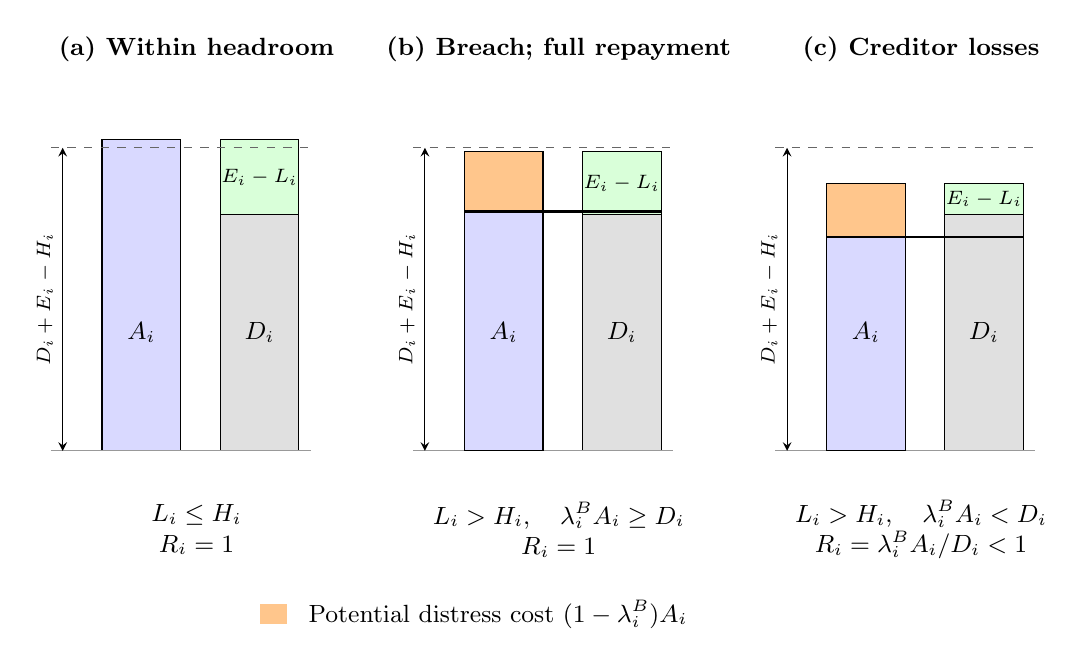
\begin{tikzpicture}[x=1cm,y=1cm,>=stealth,font=\small]
% Common illustrative values: D=3, E=1, H=.15, lambda=.8.
\foreach \shift/\height/\title in {0/3.95/{(a) Within headroom},4.6/3.8/{(b) Breach; full repayment},9.2/3.4/{(c) Creditor losses}} {
 \begin{scope}[xshift=\shift cm]
  \node[font=\small\bfseries,align=center] at (1.2,5.1) {\title};
  \fill[blue!15] (0,0) rectangle (1,\height);
  \draw (0,0) rectangle (1,\height);
  \fill[black!12] (1.5,0) rectangle (2.5,3);
  \fill[green!15] (1.5,3) rectangle (2.5,\height);
  \draw (1.5,0) rectangle (2.5,\height);
  \draw (1.5,3) -- (2.5,3);
  \node at (.5,1.5) {$A_i$};
  \node at (2,1.5) {$D_i$};
  \node[font=\scriptsize] at (2,{(3+\height)/2}) {$E_i-L_i$};
  \draw[black!40] (-.65,0) -- (2.65,0);
  \draw[dashed,black!60] (-.65,3.85) -- (2.65,3.85);
  \draw[<->] (-.5,0) -- node[midway,above,sloped,font=\scriptsize] {$D_i+E_i-H_i$} (-.5,3.85);
 \end{scope}
}
\foreach \shift/\height in {4.6/3.8,9.2/3.4} {
 \begin{scope}[xshift=\shift cm]
  \fill[orange!45] (0,{.8*\height}) rectangle (1,\height);
  \draw (0,0) rectangle (1,\height);
  \draw[thick] (0,{.8*\height}) -- (2.5,{.8*\height});
 \end{scope}
}
\node[align=center] at (1.2,-1) {$L_i\leq H_i$\\$R_i=1$};
\node[align=center] at (5.8,-1) {$L_i>H_i,\quad\lambda_i^B A_i\geq D_i$\\$R_i=1$};
\node[align=center] at (10.4,-1) {$L_i>H_i,\quad\lambda_i^B A_i<D_i$\\$R_i=\lambda_i^B A_i/D_i<1$};
\fill[orange!45] (2,-2.2) rectangle (2.35,-1.95);
\node[anchor=west,font=\small] at (2.5,-2.075) {Potential distress cost $(1-\lambda_i^B)A_i$};
\end{tikzpicture}%
}

\end{figure}
